% $Id: chapter4.tex 1790 2010-09-28 16:46:40Z jabriffa $

\chapter {System Design}

\section{Prototype}
The prototype mostly consisted of the user being able to create an account, and create posts that simply included a text. As stated before, since I decided to use Django to develop this app, I had to work with apps. This means that every major aspect of the project such as blog posts and account of is implemented as an app. During this process, the agile design methodology played a big role in the constant reimplemntations. In order to design and implement the different parts of the protoype such as user accounts, the agile methodology made it easier to concentrate on one thing at a time through heaps.

\begin{figure}[htbp]
\begin{minipage}[t]{0.45\linewidth}
    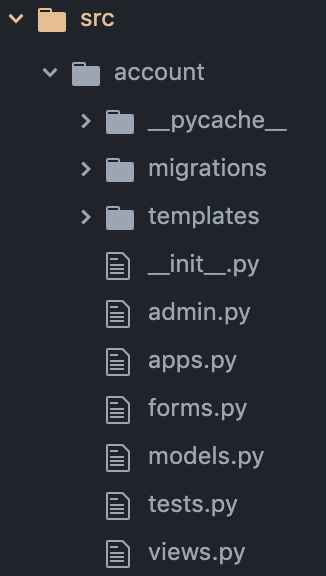
\includegraphics[scale=0.5]{Figures/apps_django}
    \caption{Django app file layout}
    \label{apps_django}
\end{minipage}%
    \hfill%
\begin{minipage}[t]{0.45\linewidth}
    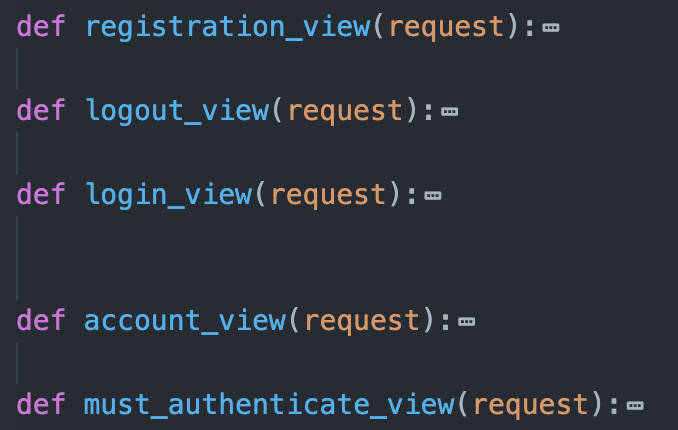
\includegraphics[width=\linewidth]{Figures/account_view}
    \caption{Account view methods}
    \label{account_view}
\end{minipage}
\end{figure}

In Figure \ref{account_view} are the methods implemented during the prototype process that handled the account authentication.

\section{User Interface Design and Usability}

\begin{figure}[htbp]
\begin{minipage}[t]{0.45\linewidth}
    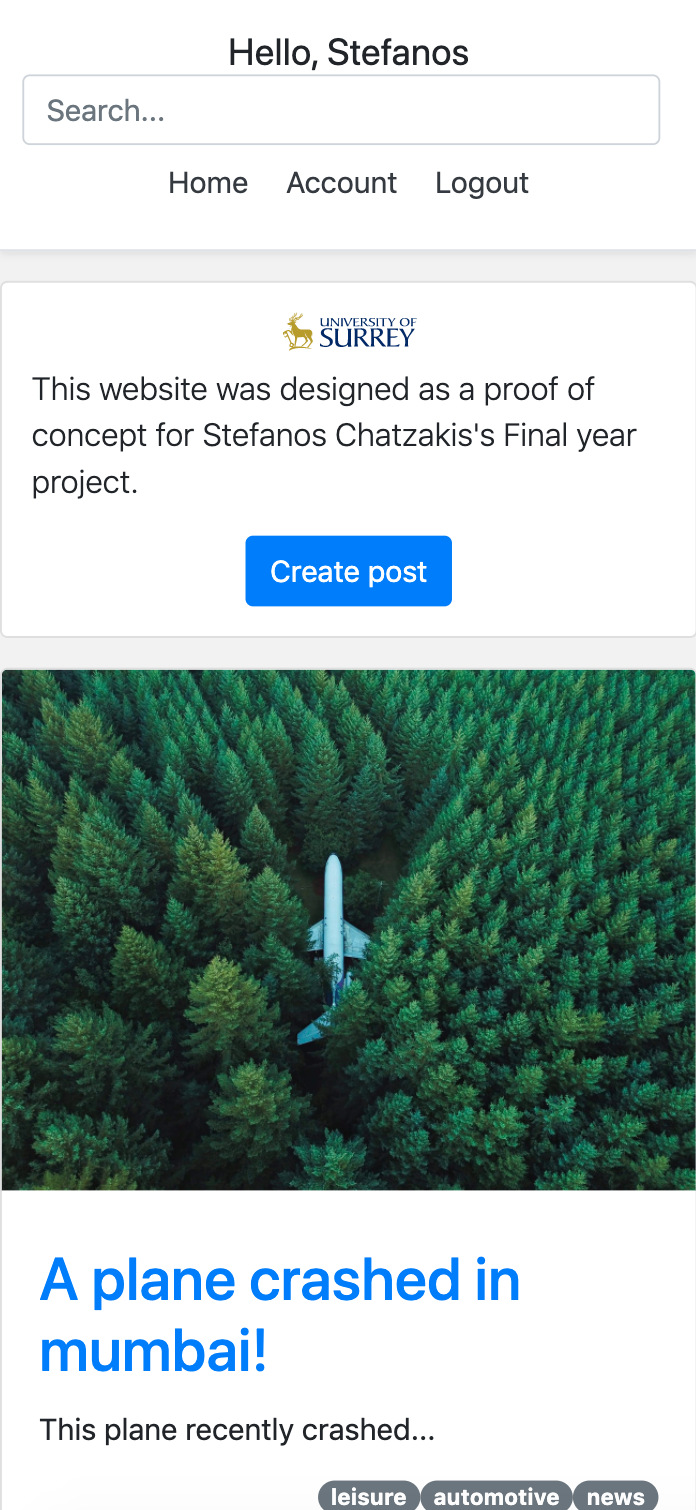
\includegraphics[width=\linewidth]{Figures/home_mobile}
    \caption{Home page from mobile device}
    \label{home_mobile}
\end{minipage}%
    \hfill%
\begin{minipage}[t]{0.45\linewidth}
    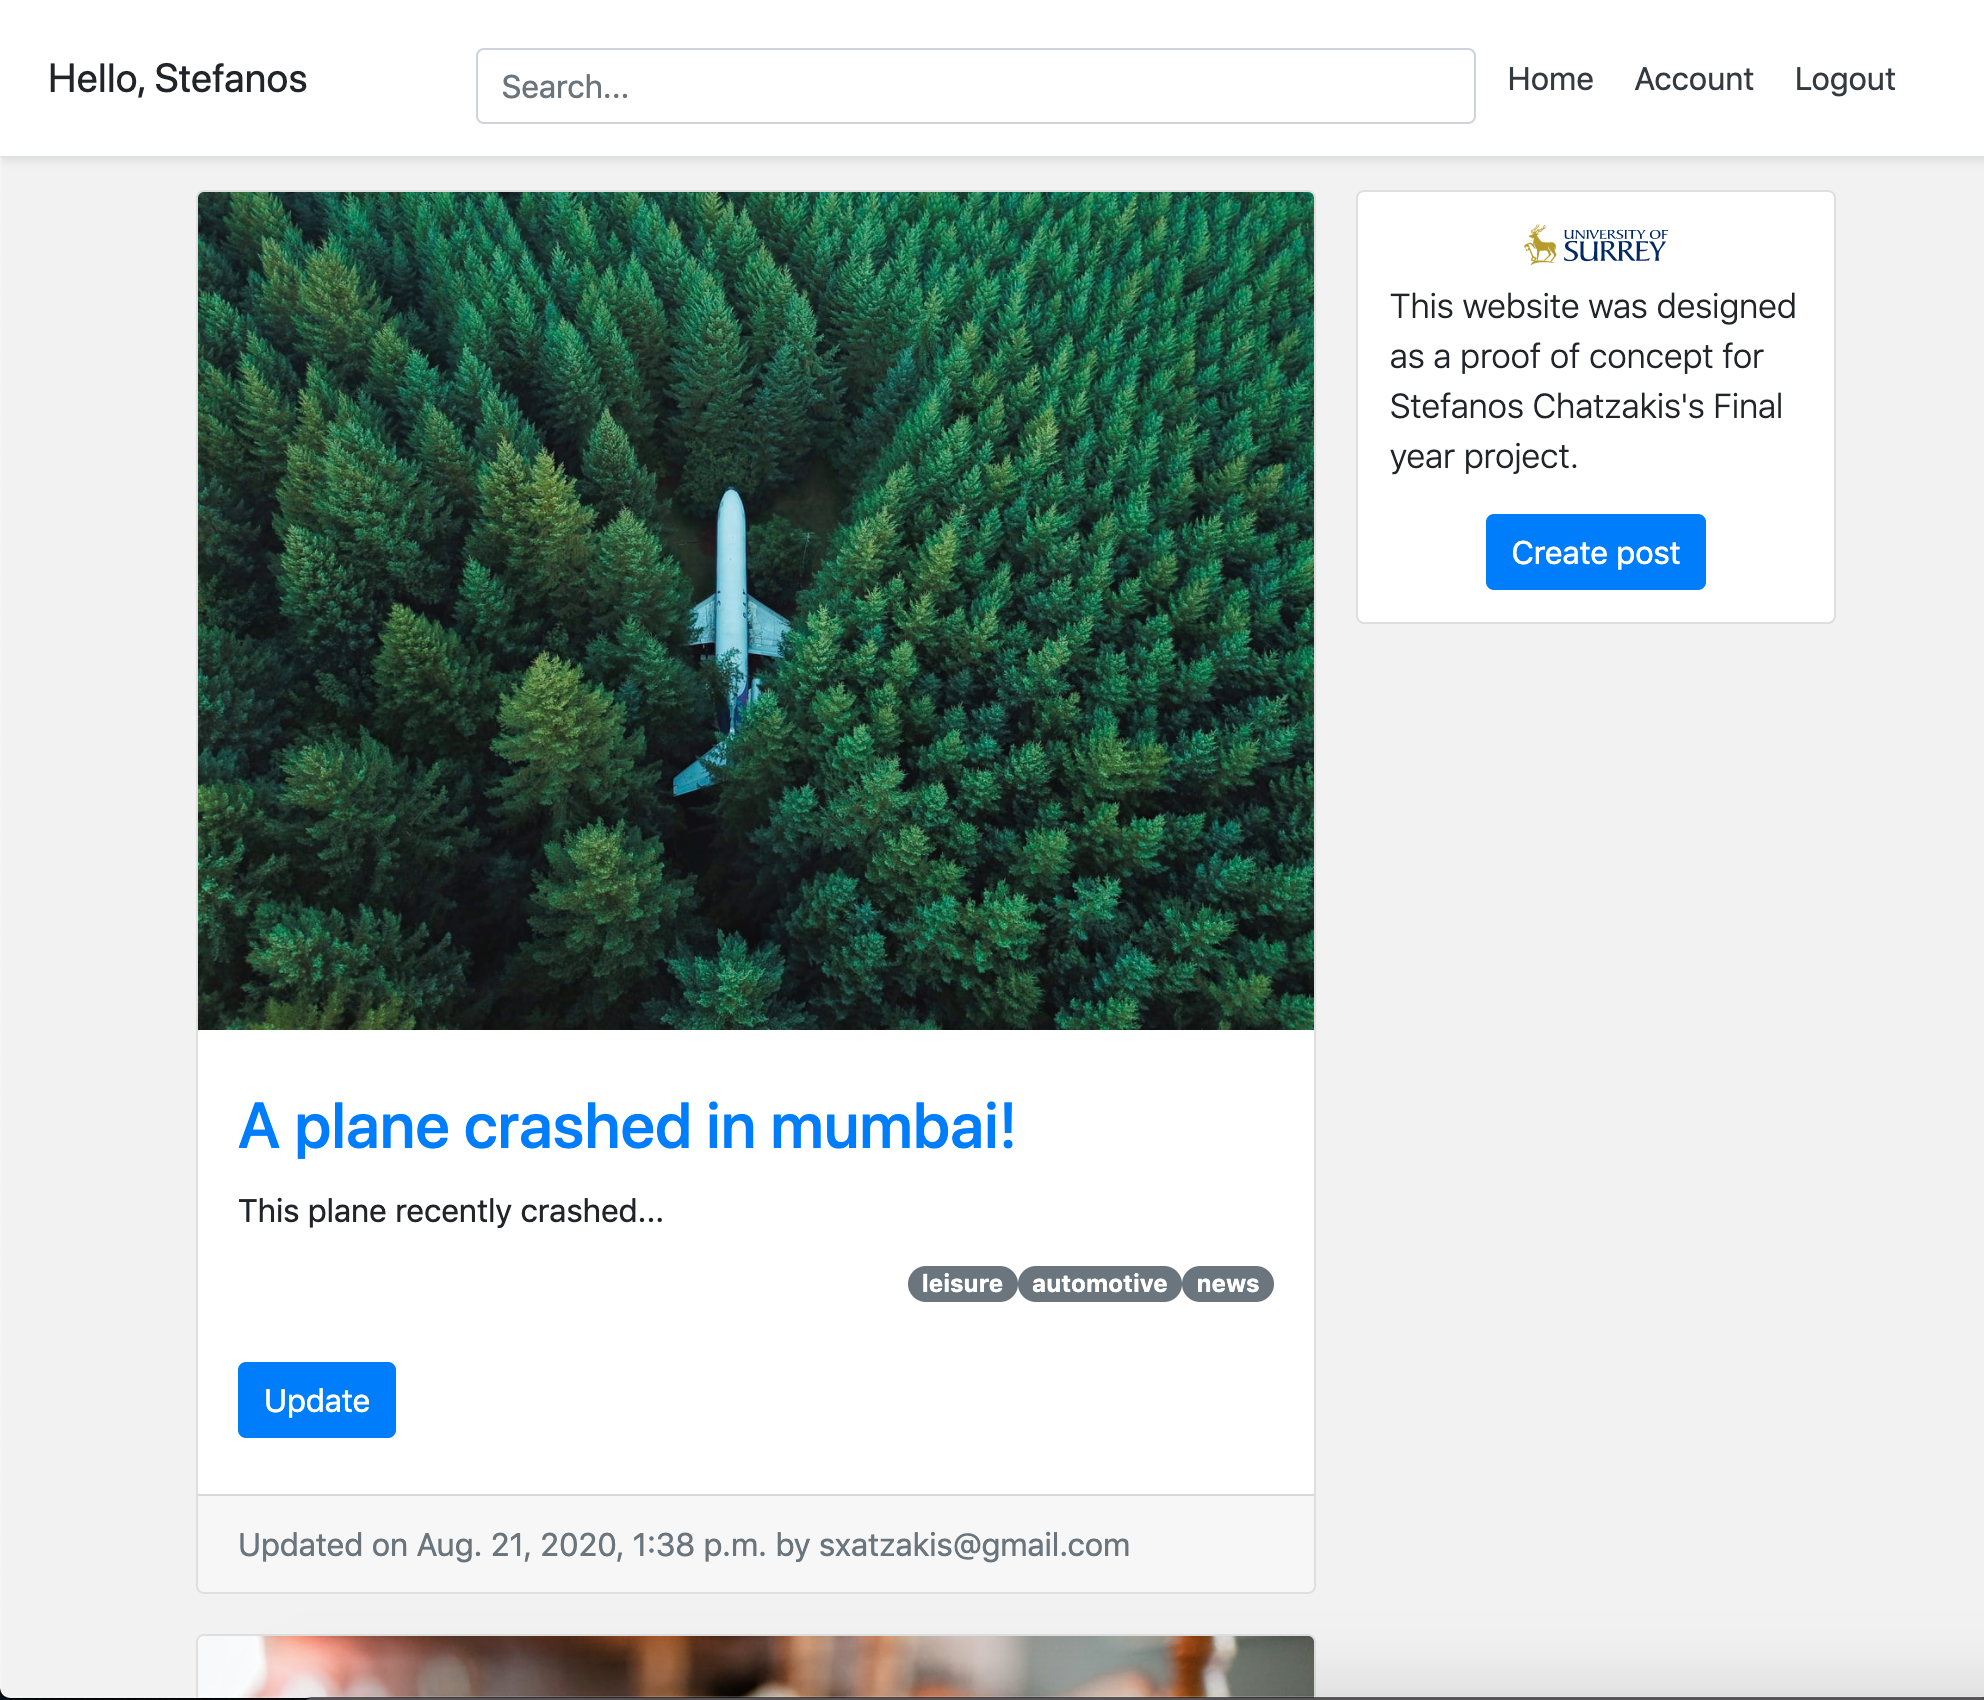
\includegraphics[width=\linewidth]{Figures/home_pc}
    \caption{Home page from desktop}
    \label{home_pc}
\end{minipage}
\end{figure}

During the system analysis, I touched upon the user experience, both in how the user should interact with the colours and buttons and when a certain colour should be used. This section explains how those principles where implemented in the final version of the project. The project is designed to work in a plethora of screen sizes as seen on \ref{home_mobile} and \ref{home_pc} making the project responsive giving the algorithm the chance to stand out, while providing an enjoyable experience to the user.

\subsection{Home Page}

\ref{home_pc} shows the home page view of the website. It consists of the template mentioned in the system analytics, and the rest of the website follows along with those characteristics. The page header, includes a welcoming message, a search bar and three buttons which vary, depending on if the user is logged in or not. These buttons include: "Home", "Account" or "Login" and "Logout" or "Register". Then we can see the main content, which includes the blog post that is implemented as mentioned before and the create post section which again, follows the user experience philosophy mentioned before.

\subsection{Account Page}

\begin{figure}[htbp]
\begin{minipage}[t]{0.45\linewidth}
    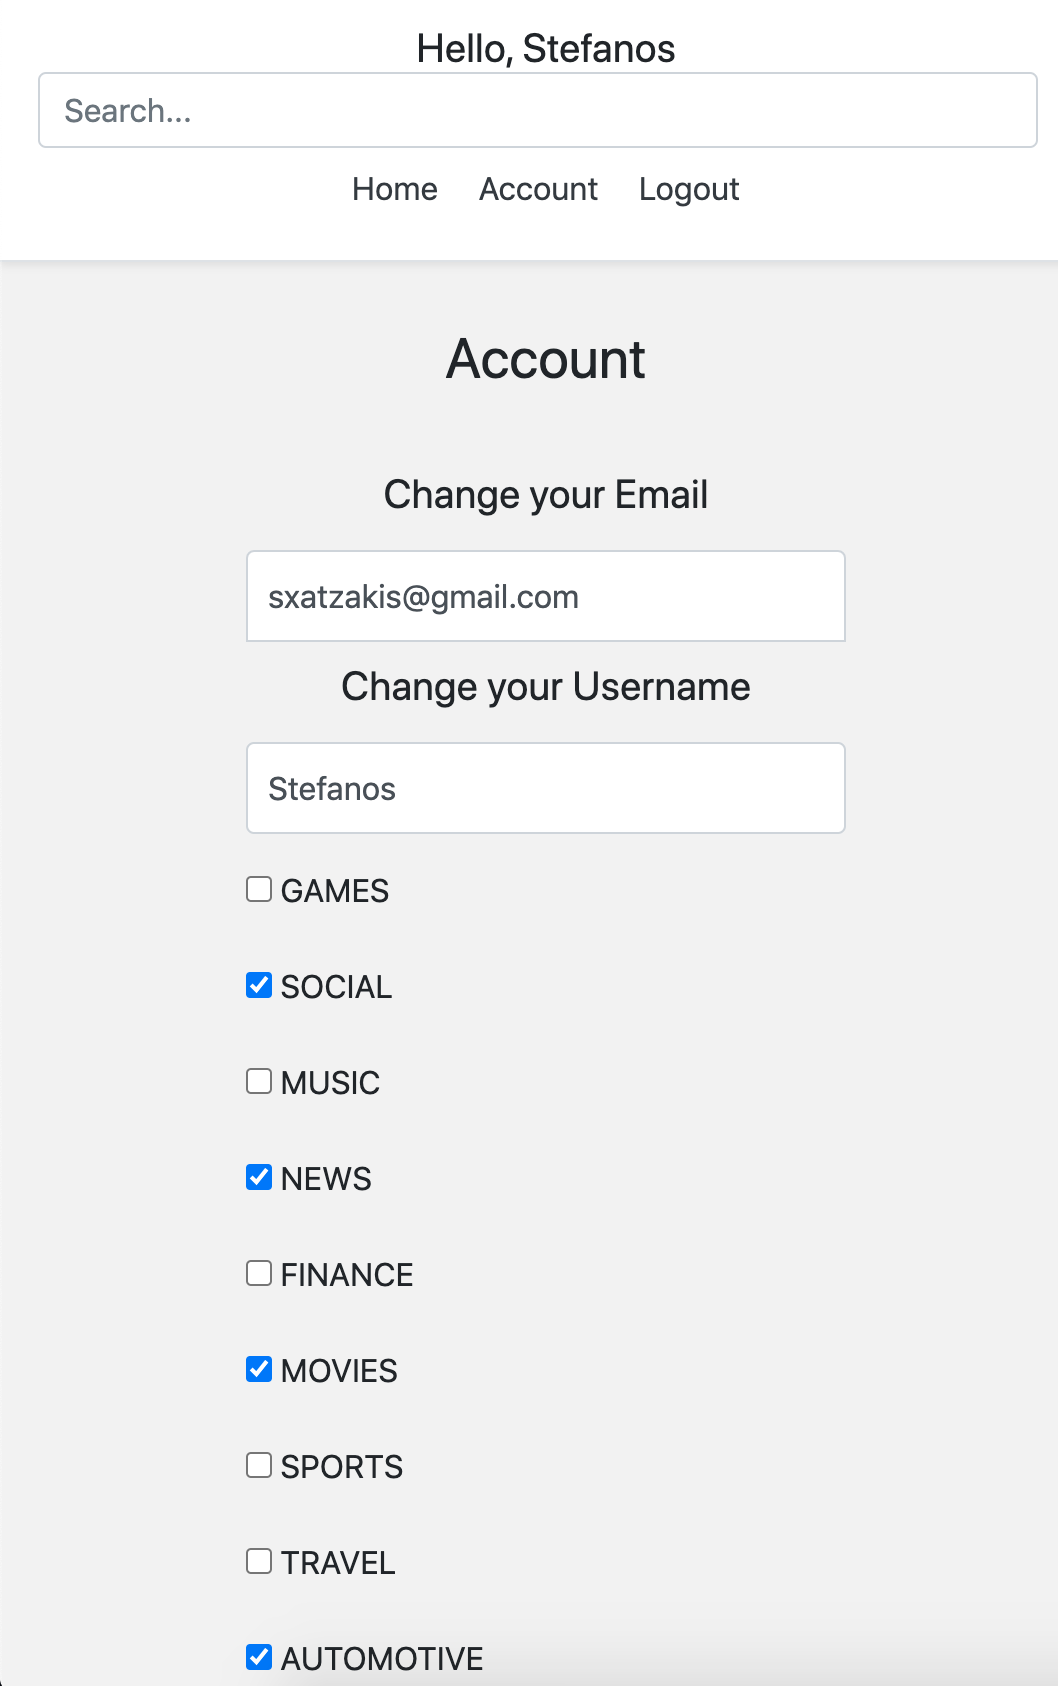
\includegraphics[width=\linewidth]{Figures/account_1}
    \caption{Account page pt. 1}
    \label{account_1}
\end{minipage}%
    \hfill%
\begin{minipage}[t]{0.45\linewidth}
    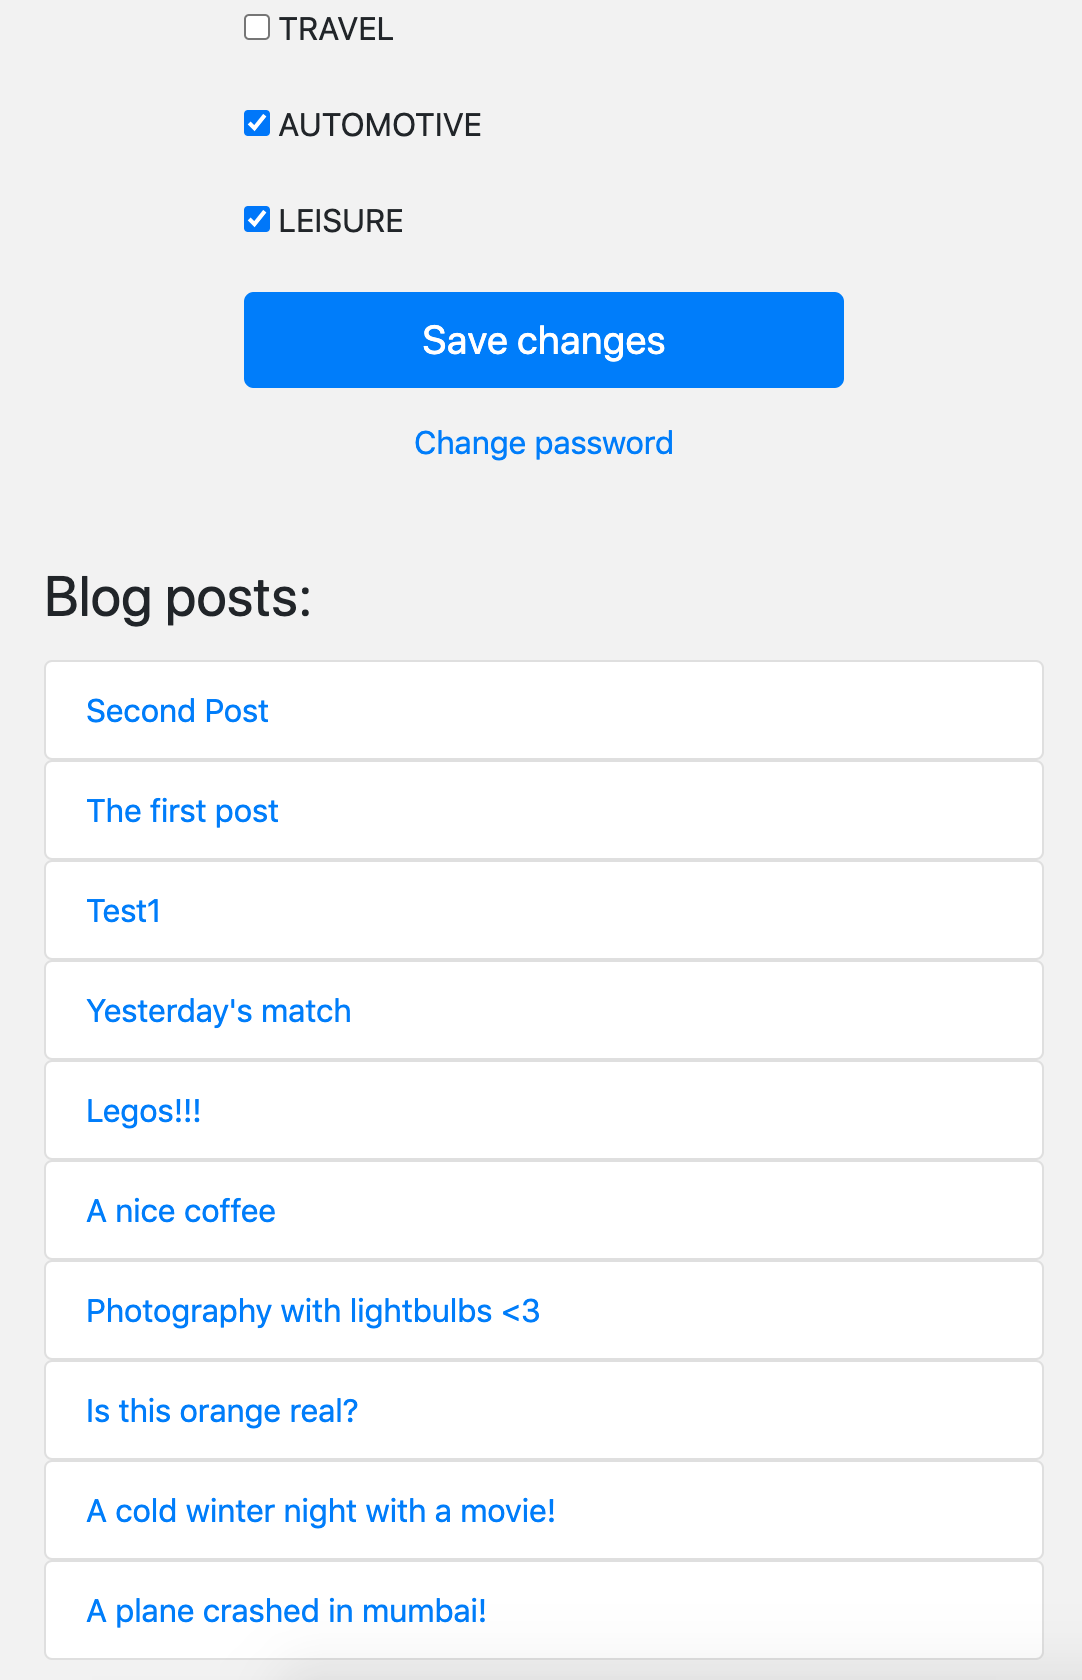
\includegraphics[width=\linewidth]{Figures/account_2}
    \caption{Account page pt. 2}
    \label{account_2}
\end{minipage}
\end{figure}

\ref{account_1} and \ref{account_2} display the account page. Apart from the header which hasn't changed, the main page content has changed, and several fields are visible. In this page, the user can edit their personal information (which is securely handled by Django's authentication system); as well as configure their interests and view all the posts they have made. This page also follows the consistent design decisions mentioned before.

\section{Difficulties faced}
This part will mainly touch upon difficulties faced during the development process of designing and implementing the program.

\subsection{Pre-development}
During the planning process, the choice to use Django was certainly not one without issues. For example, there isn't much information online to create a form that handles the information the way I needed them to and how to render them effectively. These issues mostly have to be learned through trial and error with the Django documentation being the sole guide. This resulted in spending a lot of time to learn all the Django components before the implementation could begin. Still, since many big organisations such as Reddit run their website entirely on the Django framework, it made me confident that the learning curve was worth it.

\subsection{Development}
During the development process, I did come across a few issues, mostly regarding keeping track of versions from different dependencies and programs which sometimes resulted in restarting the project. During the designing process, there were parts of the project that needed re-implementation for a variety of reasons, like UI, and sorting issues. Reflecting back to these issues, it is more apparent that the reimplementation process of different parts of the algorithm, provided a valuable learning opportunity which led to me writing more efficient code overall.
